
\section{Ejercicio 2.}

\subsection{Parte a.}

\par Exploramos diferentes layouts para visualizar la red delfines.
En la figura \ref{fig:Layout_delfines} observamos el resultado de graficar
el grafo con el Fruchterman - Reingold layout. 
\par El algoritmo para realizar este layout se basa en asignarles fuerzas de interacción ficticias a los nodos. Típicamente se basa en que los nodos ligados tengan una fuerza de atracción análoga a la fuerza de un resorte, sumado a una fuerza de repulsión entre todos los nodos, análoga a la interacción coloumbiana entre partículas cargadas idénticamente.
\par Este tipo de layout nos permitió visualizar la existencia de dos comunas de delfines, ligadas a través de unos pocos nodos.

\begin{figure}[h]
\centering
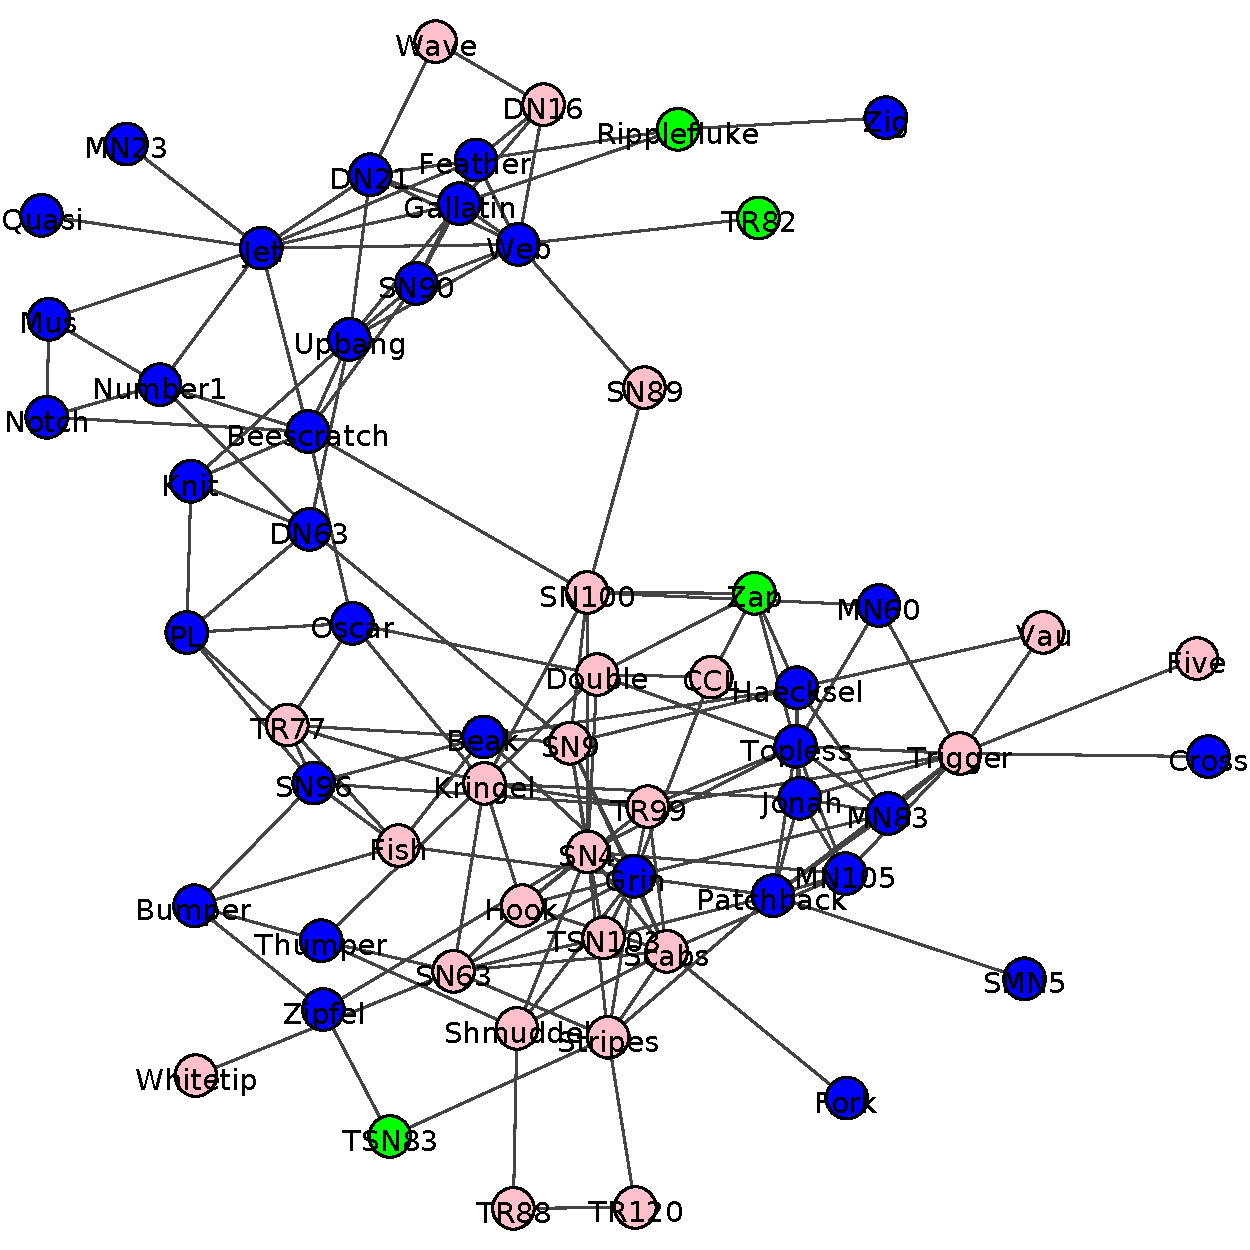
\includegraphics[scale = 0.50]{figuras/FrutRein}
\label{fig:Layout_delfines}
\caption{Fruchterman - Reingold layout. Los colores de los nodos se refieren al sexo del delfín: azul, macho; rosa, hembra; verde, sexo no indicado en el dataset.}
\end{figure}

\subsection{Parte b.}

\par En esta sección nos propusimos estudiar si la red era de carácter homofílica o no, es decir, si un dado nodo tiende a ligarse con nodos que comparten una caractrística con él, como es en este caso, el género de los delfines.
Para ello, se comparó la red de delfines con el género asociado con una red de misma topología pero sorteando al azar el género de los delfines. Esto constituye lo que llamamos hipótesis nula, es decir, el género de un delfín es asignado de manera totalmente independiente a la topología de la red.
\par En la red del dataset, la fracción de links entre delfines de distinto género (sin contar los pares de vértices que incluyan un delfín con género no especificado) es de $\rho_{M-F} \sim 0.32$. Manteniendo constante la topología de la red sorteamos los géneros entre los nodos, manteniendo constante la cantidad de machos, hembras, y ejemplares sin especificación de genero. Realizamos $1000000$ de realizacion, calculando la fracción de links entre géneros al final, obteniendo como resultado el histograma de la figura \ref{fig:Histograma}.
\par El valor medio de links entre géneros de la distribución obtenida es $<\rho_{M-F}>^{HN} = 0.43 \pm 0.04$, donde el error es la desviación estandar de la misma.
\par Del histograma podemos concluir que, dada la hipotesis nula, la probabilidad de que la fracción de links entre géneros sea $\sim 0.32$ es menor a $0.005$, por lo que podemos descartar la hipótesis nula, es decir, la distribución actual de links entre géneros no proviene de una distribución al azar de los mismos. Por otro lado, este número es mucho menor que el valor medio $<\rho_{M-F}>^{HN}$, lo cual indica que la mayor cantidad de links se da entre delfines del mismo género, lo cual apoya la hipótesis de que esta red es homofílica.
\par Estimación del valor medio: la probabilidad de tomar un link entre un macho y una hembra es $2 \rho_{M} \rho_{F}$, donde $\rho$ son las densidades de cada género en la red real. Entonces la probabilidad de la tomar $m$ links es:
\begin{equation}
	P(m) = {N' \choose m} (2 \rho_{M} \rho_{F})^{m} (1 - 2 \rho_{M} \rho_{F})^{N' - m}
\end{equation}
donde $N'$ es $N(N-1)/2$, el número total de links que se pueden formar en una red de $N$ nodos. El valor medio de links es entonces $<m> = N' 2 \rho_{M} \rho_{F}$, y la desviación estándar de links $std(m) = (N' 2 \rho_{M} \rho_{F} (1 - 2 \rho_{M} \rho_{F}))^{1/2}$. Para los valores del problema, obtenemos:
\begin{equation}
	<m> = 68 \pm 7 
\end{equation}

\begin{tabbing}
\hspace{5cm} \= \hspace{5cm} \kill
Observable \> Valor \\
$N$ \> $62$ \\
$N' = N(N-1)/2$ \> $1891$ \\
$\rho_{M}$ \> $0.55$ \\
$\rho_{F}$ \> $0.39$ \\
$p_{M-F}$ \> $2 \rho_{M} \rho_{F} \sim 0.43 $ \\
$<m>_{estimado}$ \> $N' p_{M-F} \sim 811$
\end{tabbing}



\begin{figure}[h]
\centering
\includegraphics[scale = 0.50]{figuras/Histograma}
\label{fig:Histograma}
\caption{Histograma}
\end{figure}

\subsection{Parte c.}

\begin{figure}
\centering
\begin{subfloat}[]
{
	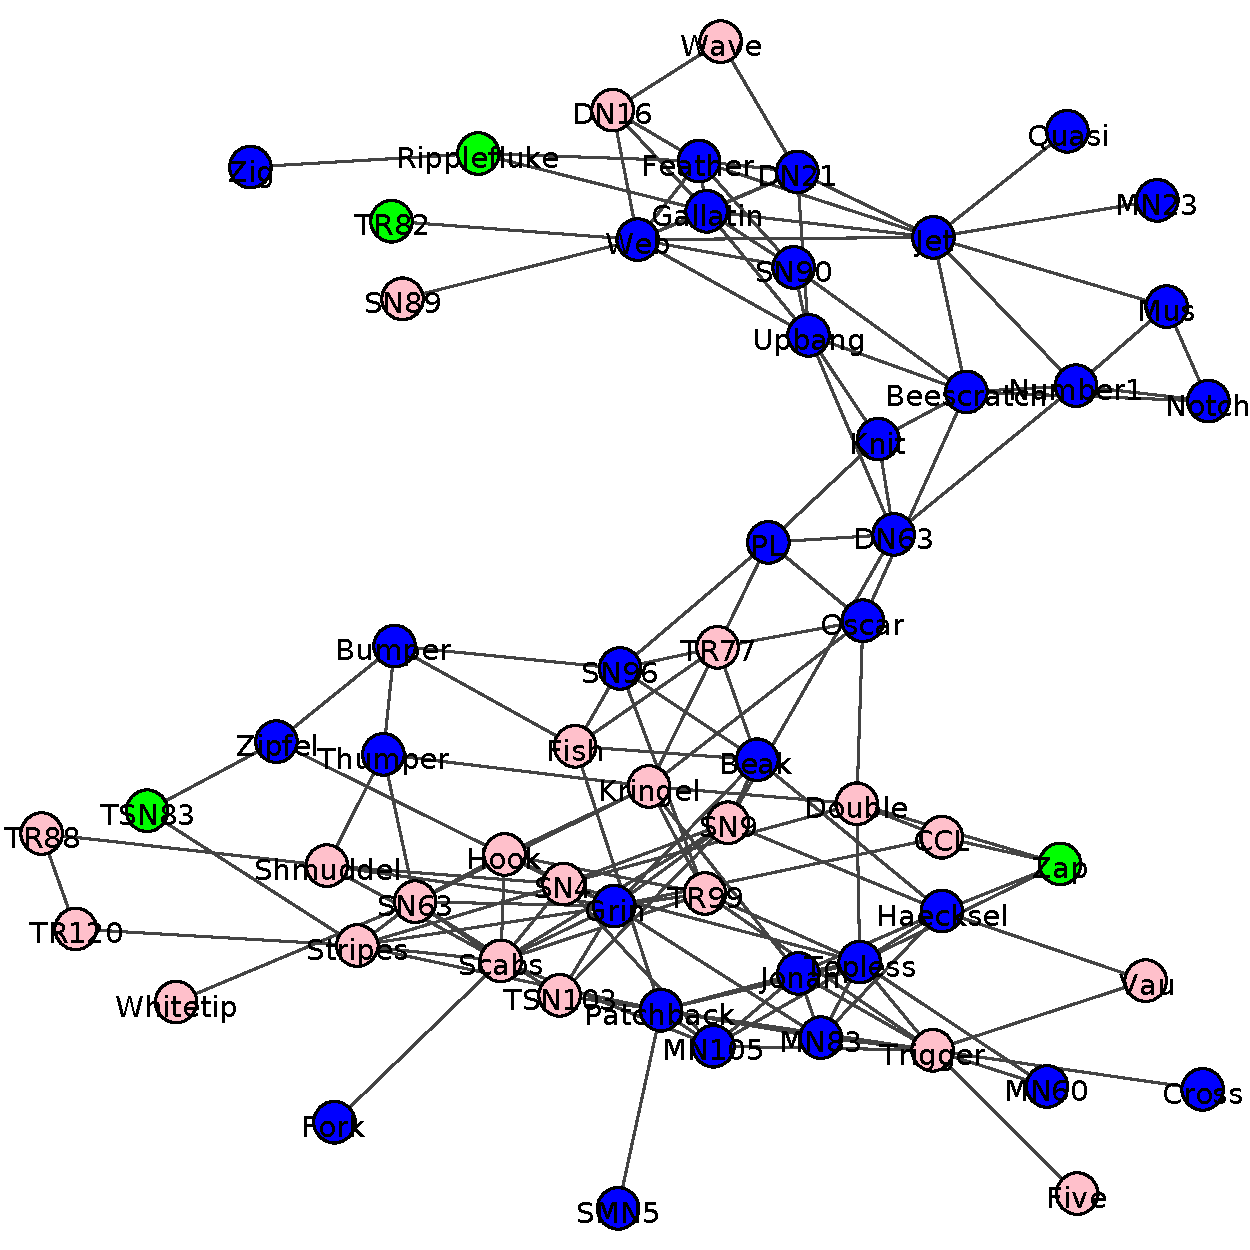
\includegraphics[scale = 0.27]{figuras/Parte_c0} 
}
\end{subfloat}
\begin{subfloat}[]
{
	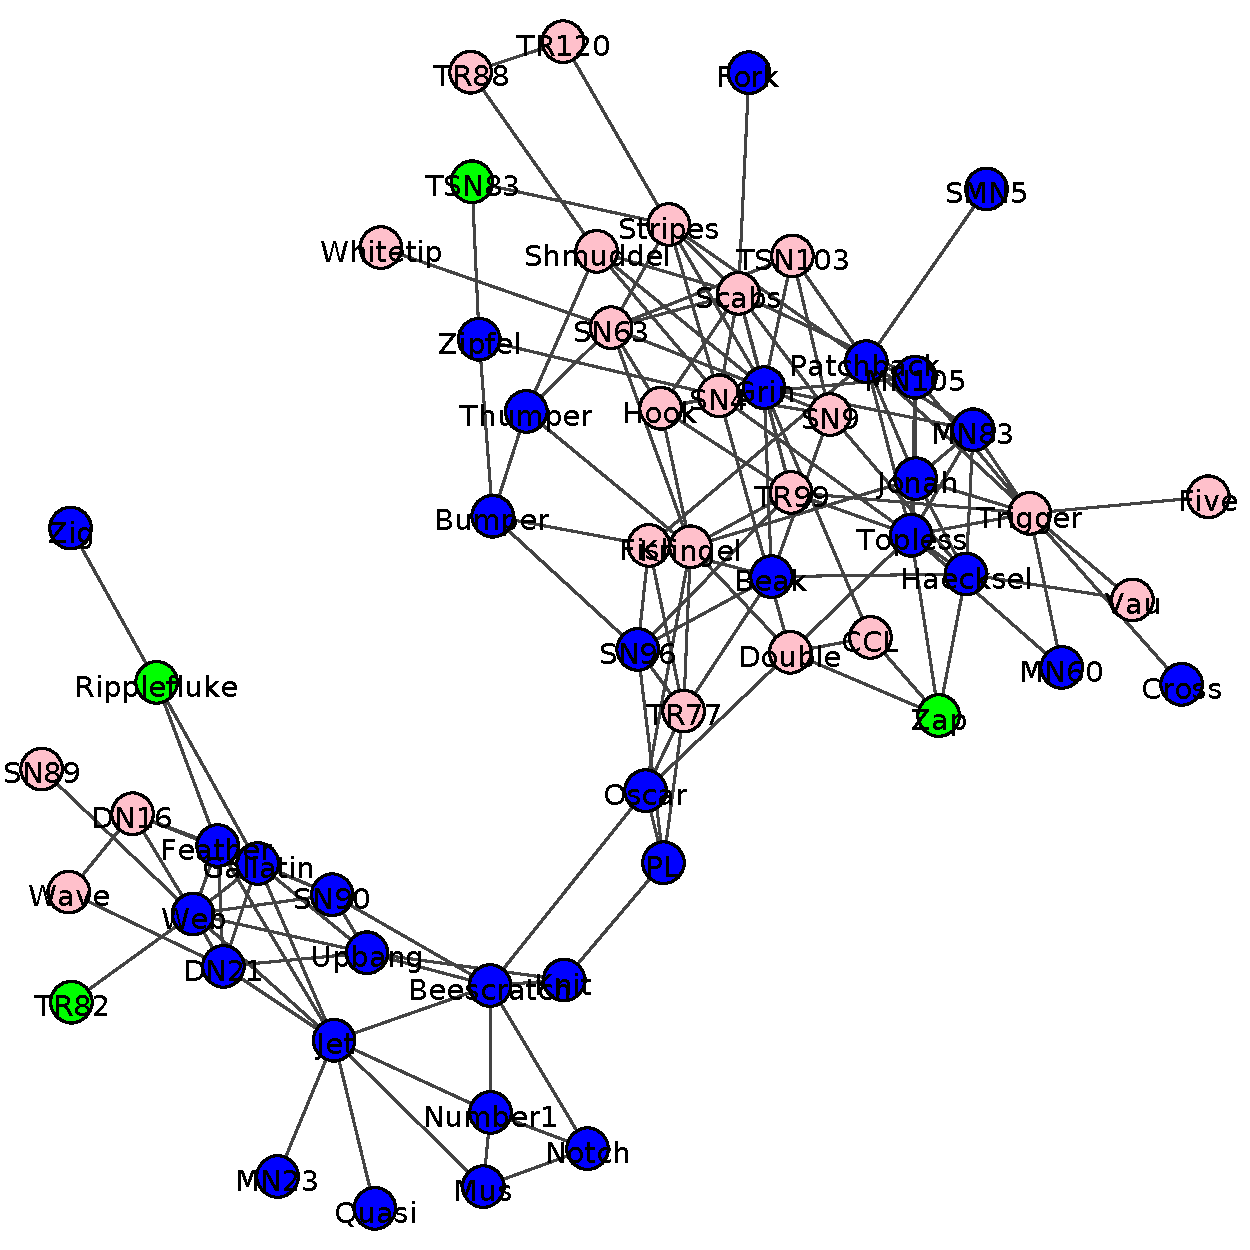
\includegraphics[scale = 0.27]{figuras/Parte_c1}
}
\end{subfloat}
\begin{subfloat}[]
{
	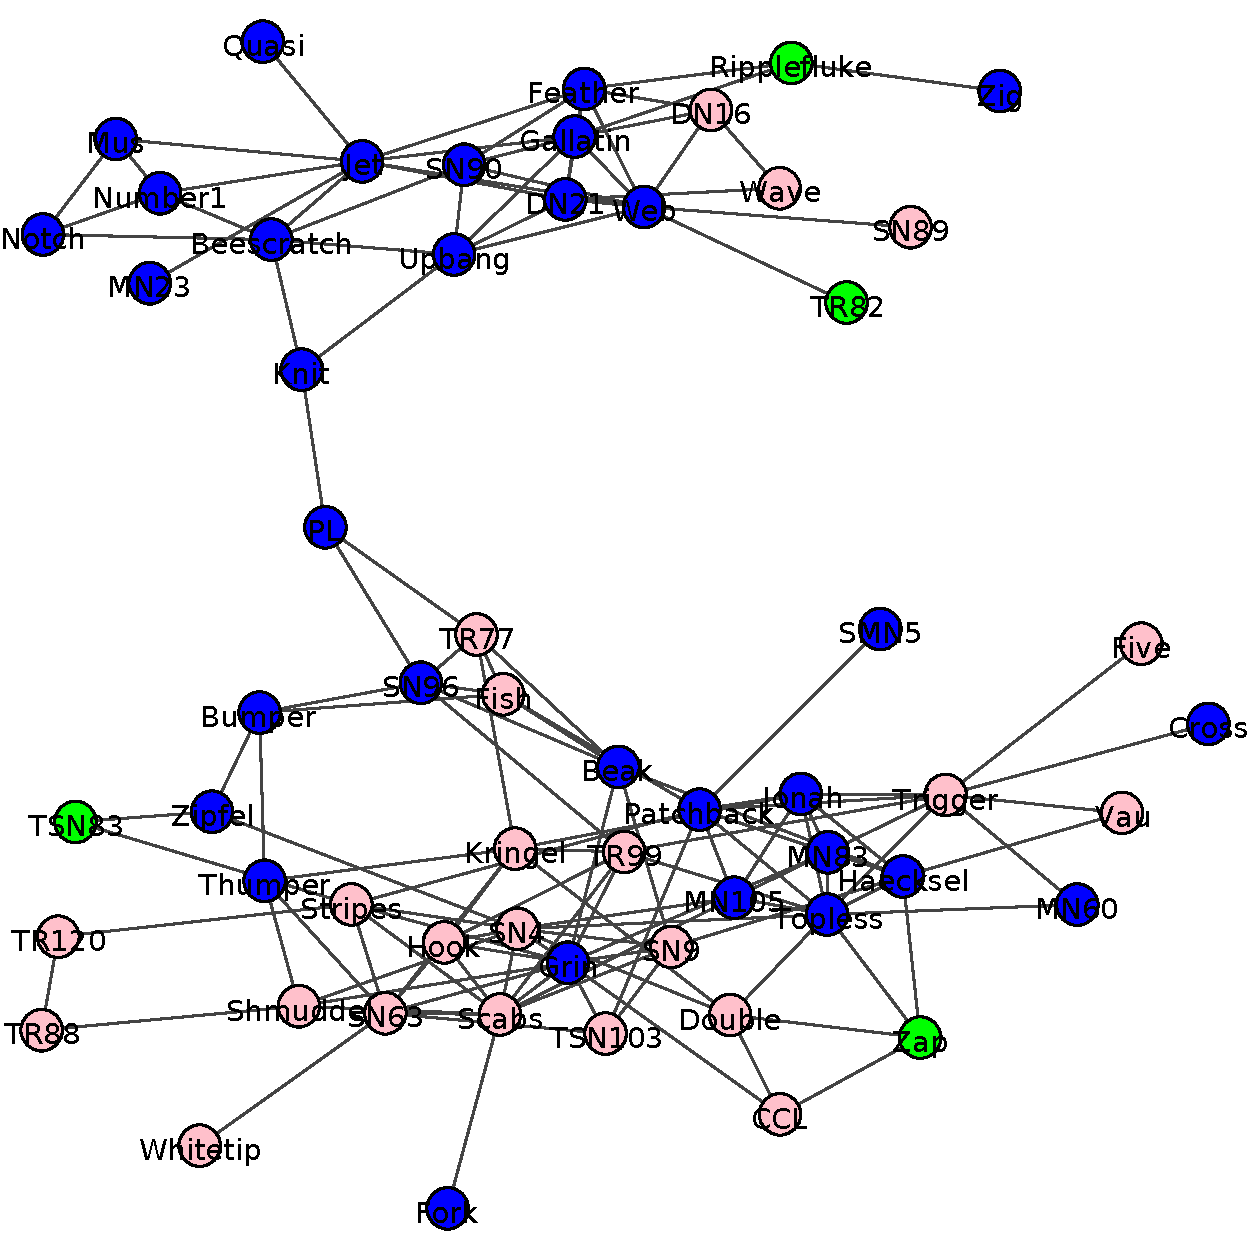
\includegraphics[scale = 0.27]{figuras/Parte_c2} 
}
\end{subfloat}
\begin{subfloat}[]
{
	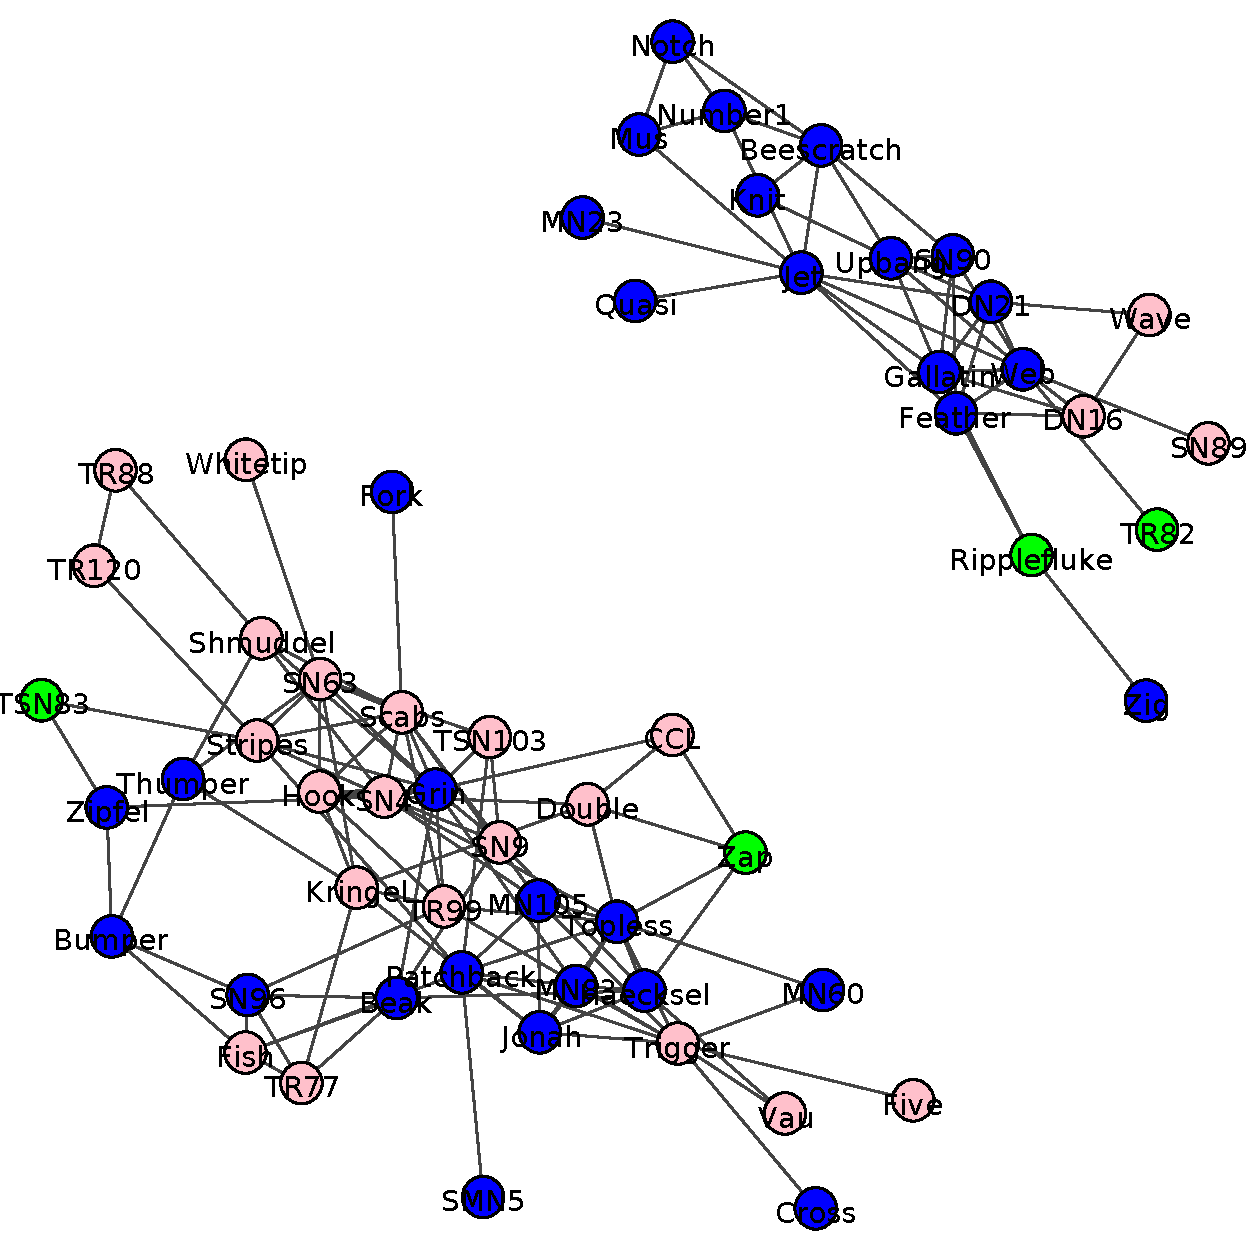
\includegraphics[scale = 0.27]{figuras/Parte_c3} 
}
\end{subfloat}
\label{fig:Betweennes}
\caption{Fruchterman - Reingold layout. Los colores de los nodos se refieren al sexo del delfín: azul, macho; rosa, hembra; verde, sexo no indicado en el dataset.}
\end{figure}
